\chapter{Fundamentals of Computer Design}

\section{Power Consumption Evaluation}
In CMOS technology, power consumption is absorbed passively and actively. In the former case, power absorption is a symptom of inevitable current leakages between transistors' junctions, while in the latter case, current is drawn by logic gates when charging and discharging during operation and switching which, as a matter of fact, also causes transient short circuits, i.e. the control signal has finite slope and the N-MOS and P-MOS transistors won't switch perfectly in sync. 

\begin{figure}[htbp]
    \centering
    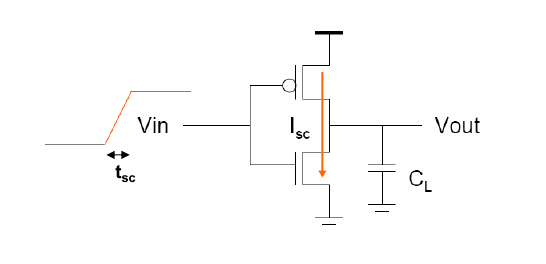
\includegraphics[width=0.7\textwidth]{images/logic_gate_1}
    \caption{Representation of a Logic Gate during a transient short-circuit: both transistors are conducting, creating a direct path to ground. $C_L$ is a parasitic capacitance responsible for most of the active energy consumption.}
    \label{fig:my_label}
\end{figure}

Active (or Dynamic) power consumption of a transition ($E_t$) is calculated by multiplying the energy necessary to switch state times the probability of this event (dependent for instance on the architecture). Power, being energy over time, equals energy times clock frequency.
\begin{align*}
E_t &= C_L \cdot V_{DD}^2 \cdot P_{0 \rightarrow 1} \\
\textrm{Power} &= C_L \cdot V_{DD}^2 \cdot P_{0 \rightarrow 1} \cdot f_{0 \rightarrow 1} = E_t \cdot \textrm{Frequency}
\end{align*}

Additionally, one needs to account for the mentioned short-circuits, absorbing a current proportional to the rising time of the signal $t_{sc}$:
\begin{align*}
E_{sc} &= t_{SC} \cdot V_{DD} \cdot I_{peak} \cdot P_{0 \rightarrow 1} \\
\textrm{Power} &= t_{sc} \cdot V_{DD} \cdot I_{peak} \cdot P_{0 \rightarrow 1} \cdot f_{0 \rightarrow 1} = E_{sc} \cdot f_{0 \rightarrow 1}
\end{align*}

Overall, dissipated power is given by the combination of:
\begin{itemize}
    \item $E_t$, mainly dependent on parasitic capacitance, therefore on number of gates and transistor size
    \item $E_{sc}$, dependent on transistor technology, size, temperature, and signal slope
    \item $E_{leakage} = V_{DD} \cdot I_{leakage}$, increasing with higher temperatures and lower threshold voltages
    \item $\textrm{Frequency}$, dependent on performance
    \item $P_{0 \rightarrow 1}$, dependent on signal statistics
\end{itemize}

Therefore:
\begin{align*}
    \textrm{Power} =&\ C_L \cdot V_{DD}^2 \cdot P_{0 \rightarrow 1} \cdot f_{0 \rightarrow 1}\\
    &\ + t_{sc} \cdot V_{DD} \cdot I_{peak} \cdot P_{0 \rightarrow 1} \cdot f_{0 \rightarrow 1}\\
    &\ + V_{DD} \cdot I_{leakage}
\end{align*}


\section{Cost Estimation}
Costs tend to generally decrease due to a number of factors. Manufacturing yield $Y$ for example, increases even without improvements in the implementation technology, adding up to an increase in production volumes which result in more amortized manufacturing costs. Costs trends also decrease because of competition effects, requiring selling prices to be close to production ones.

Experimentally, the cost $C$ of an integrated circuit is given by:
$$C=\frac{C_{die} + C_{testing} + C_{packaging}}{Y}$$
\noindent where $C_{die}$ is the cost of manufacturing a die, $C_{testing}$ that of testing a die after cutting it from a wafer, and $C_{packaging}$ that of packaging and testing the working ones. Unlike these last two costs which solely depend on the complexity of the IC, $C_{die}$ depends on more factors:
$$C_{die}=\frac{C_{wafer}}{N_{die} \cdot Y_{die}}$$
Where $N_{die}$, in turn, equals the number of dies on a round wafer of diameter $D$, minus those close to edge:
$$N_{die}=\frac{\textrm{Area of wafer}}{\textrm{Area of die}} - \textrm{Chips near the edge} = \frac{\pi \cdot \frac{1}{4} D^2}{A_{die}} - \frac{\pi \cdot D}{\sqrt{2 \cdot A_{die}}}$$
And $Y_{die}$ is given by:
$$Y_{die}=Y_{wafer} \cdot \left(1 + \frac{N_{defects} \cdot A_{die}}{\alpha}\right)^{-\alpha}$$
\noindent with $N_{defects}$ being the number of defects per unit area of the wafer, and $\alpha$ an empirical value related to manufacturing complexity.
\newline

In conclusion, it can be inferred that a designer only has control on the strong dependence that $A_{die}$ has on costs, while all other parameters only depend on the manufacturing process.


\section{Performance Evaluation}
...

\section{Design of Computing Systems}
...

